%% ===========================================================================
%% AMSE PhD thesis — main file.
%%
%% Compile with pdfLaTeX + biber.  On Overleaf: Menu -> Compiler -> pdfLaTeX,
%% Main document -> these.tex.  Locally: latexmk -pdf these.tex
%%
%% You should not need to edit the two \input lines marked GENERATED below.
%% Everything else in this file is yours.
%% ===========================================================================
\documentclass{amse_these}

%% ---------------------------------------------------------------------------
%% preamble-extra.tex — YOUR preamble additions.
%%
%% This file is never overwritten by the import script. Put here anything your
%% papers need that `amse_these.cls` does not already load.
%%
%% What is below is the set of packages and macros that working-paper preambles
%% in economics need most often. It is loaded by default because a missing one
%% usually fails *silently*: LaTeX prints "Undefined control sequence", keeps
%% going, and the symbol simply never appears in the PDF. Comment out whatever
%% you do not need.
%%
%% After running tools/import_chapter.py, read its report: it lists every
%% package your paper's own preamble loaded that is not available here.
%% ---------------------------------------------------------------------------

%%% --- Significance stars from esttab / estout ------------------------------
%% Tables exported by Stata's esttab use \sym{**}. Without it the stars vanish.
\providecommand{\sym}[1]{\ensuremath{^{#1}}}

%%% --- Numbers and units -----------------------------------------------------
\RequirePackage{siunitx}                    %% \num{12345} -> 12 345
\providecommand{\euro}{\texteuro}

%%% --- Maths shorthands commonly used in papers ------------------------------
\RequirePackage{bbm}                        %% \mathbbm{1} (indicator function)
\providecommand{\E}{\ensuremath{\mathbb{E}}}
\providecommand{\dln}[1]{\ensuremath{\mathrm{d}\ln #1}}

%%% --- Draft annotations ------------------------------------------------------
\RequirePackage[normalem]{ulem}             %% \sout{...}, \uwave{...} (latexdiff)
\RequirePackage{comment}                    %% \begin{comment} ... \end{comment}
\providecommand{\red}[1]{{\color{red}#1}}
\providecommand{\blue}[1]{{\color{blue}#1}}

%%% --- Figures drawn in TikZ / pgfplots ---------------------------------------
%% Comment this block out if none of your chapters draws figures in code:
%% it is the slowest part of this file to load.
\usetikzlibrary{trees, positioning, shapes.geometric, arrows.meta,
    decorations.pathreplacing, calc, backgrounds, fit}
\RequirePackage{pgfplots}
\pgfplotsset{compat=1.18}

%%% --- Theorem-like environments the class does not define --------------------
%% amse_these.cls already defines: theorem, assumption, corollary, proposition,
%% lemma, conjecture, algorithm, example, remark, proof.
%% Do NOT load amsthm here: it redefines `proof` and clashes with the class.
\newenvironment{prediction}%
    {\par\medskip\noindent\textbf{Prediction.}\itshape}%
    {\par\medskip}

%%% --- Colours ----------------------------------------------------------------
\definecolor{navyblue}{rgb}{0.0,0.0,0.5}
          %% your own packages and macros
%% GENERATED by tools/import_chapter.py — do not edit.
%% Empty until you run the script: put your Overleaf exports in chapters/ first.
     %% GENERATED by tools/import_chapter.py

\begin{document}
										%% title page
	\chead{}
	\pdfbookmark[0]{Thesis}{titre}
	\thispagestyle{empty}
	\newgeometry{margin=2em}

\begin{center}
	\begin{minipage}[c]{.5\linewidth}
		\raggedright
\includegraphics[height=5em]{logo/logo_amu.pdf}
	\end{minipage}\hfill
	\begin{minipage}[c]{.5\linewidth}
		%% second logo, if your thesis is a cotutelle:
		%\raggedleft\includegraphics[height=5em]{logo/partner.pdf}
	\end{minipage}\hfill
\end{center}

\vspace{1em}

\begin{center}
	\begin{minipage}[c]{.63\linewidth}
		\dhorline{\textwidth}{4pt}
	\end{minipage}\hfill
	\begin{minipage}[c]{.35\linewidth}
		\raggedleft\titl{NNT/NL : XXXXAIXMXXXX/XXXEDXXX}
		%% TODO — your numero national de these (NNT) and numero local (NL),
		%% both from https://depot-theses.univ-amu.fr/
	\end{minipage}\hfill
\end{center}

\doublespacing
\begin{flushleft}
    \titb{\HUGE\textcolor{blueamu}{THÈSE DE DOCTORAT}}\\
	\titl{\Large Soutenue à Aix-Marseille Université}\\
	%\titl{\Large dans le cadre d'une cotutelle avec }\\
	\titl{\Large le JJ MOIS AAAA par}\\ %% TODO — defence date
\end{flushleft}
\vspace{2em}
\begin{center}
	\titsb{\Huge Prénom NOM}\\ %% TODO
    \vspace{1em}
	\titm{\LARGE Title of the thesis}\\ %% TODO
\end{center}
\singlespacing

\vspace{1.5em}

\begin{center}
	\begin{minipage}[t]{.45\linewidth}
    	    \vspace{.5em}
        	\titb{Discipline}

        	\titl{Sciences Economiques}

    	    \vspace{1em}
        	\titb{École doctorale}

        	\titl{Sciences Economiques et Gestion (372)}

    	    \vspace{1em}
        	\titb{Laboratoire/Partenaires de recherche}

        	\titl{Aix-Marseille School of Economics}
			%% add other labs or partners on their own line
	\end{minipage}\hfill
	\begin{minipage}[t]{.03\linewidth}
	    \dvertline{4pt}{-21em}
	\end{minipage}\hfill
	\begin{minipage}[t]{.52\linewidth}
	    \vspace{.5em}
    	\titb{\small Composition du jury}

	    \vspace{1em}
    	\titel{
        %% TODO — one line per jury member: name, then institution underneath.
        %% Roles: Rapporteur / Rapporteure, Examinateur / Examinatrice,
        %% Président(e) du jury, Directeur / Directrice de thèse, Co-directeur.
        %% Check the spelling of every institution: it is printed as given.
        \begin{tabular}{p{12em} p{9.5em}}
        	Prénom NOM & Rapporteur \\
        	Institution \\
            \\
        	Prénom NOM & Rapporteure \\
        	Institution \\
        	\\
            Prénom NOM & Examinateur \\
        	Institution \\
            \\
            Prénom NOM & Examinatrice et \\
        	Institution & Présidente du jury \\
            \\
        	Prénom NOM & Directeur de thèse \\
        	Aix-Marseille Université \\
            \\
        	Prénom NOM & Co-directrice de thèse \\
        	Aix-Marseille Université \\
        \end{tabular}
        }
	\end{minipage}\hfill
\end{center}

\vfill

\begin{center} %% logos partenaires
	\begin{minipage}[c]{.31\linewidth}
		\centering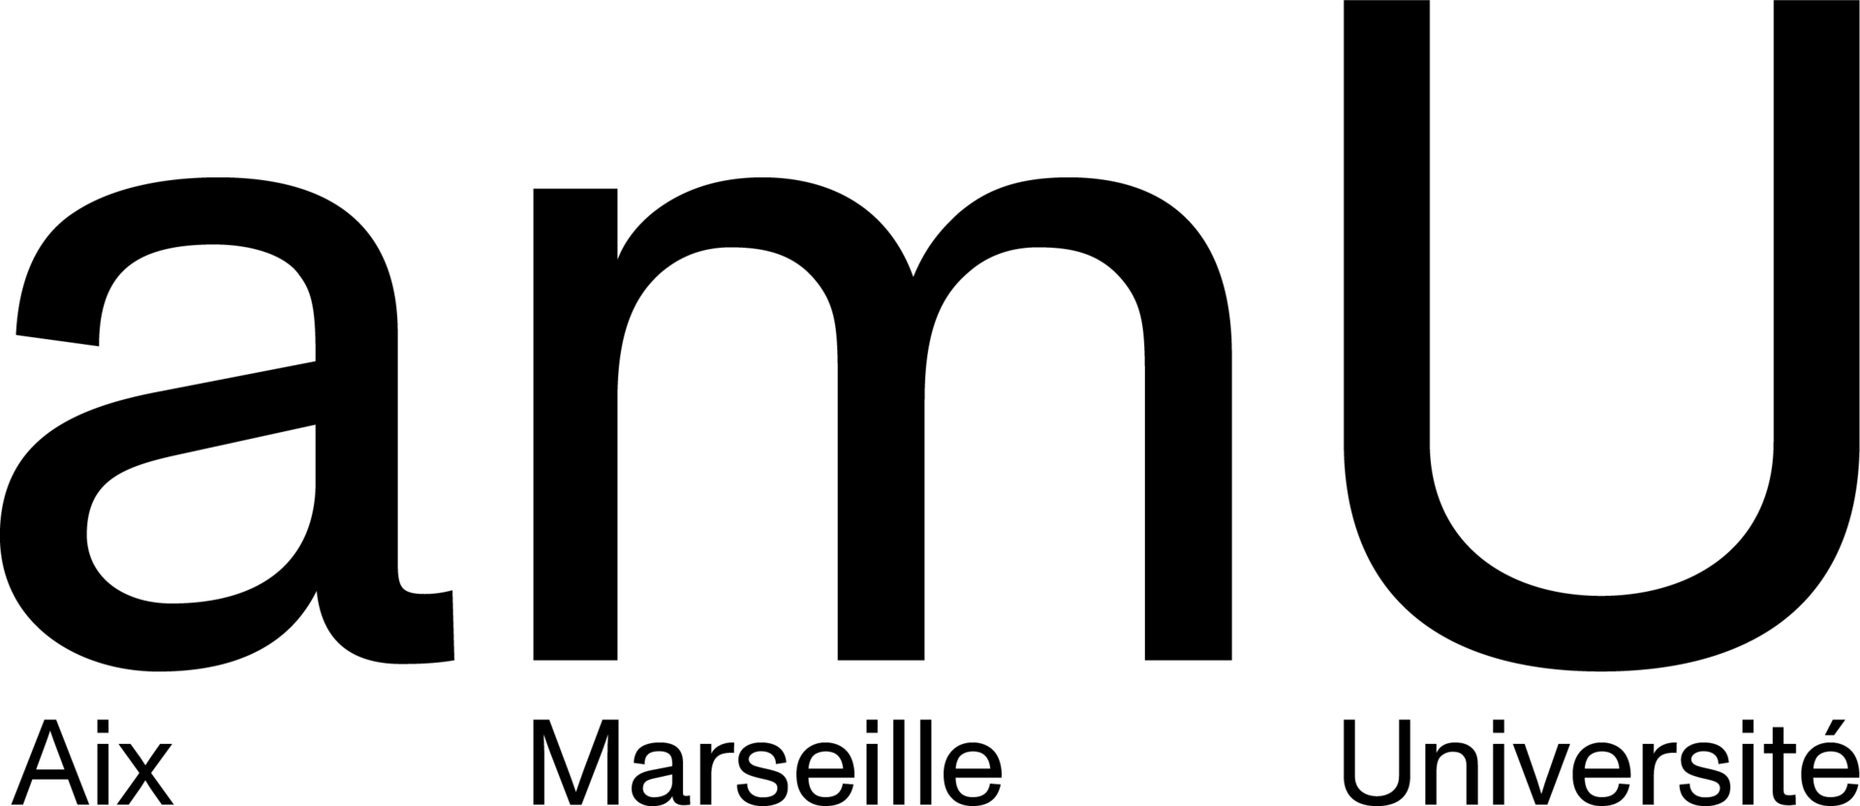
\includegraphics[width=9em]{logo/amu.png}
	\end{minipage}\hfill%
	\begin{minipage}[c]{.31\linewidth}
		\centering
\includegraphics[width=9em]{logo/amse.png}
	\end{minipage}\hfill%
	\begin{minipage}[c]{.31\linewidth}
		\centering
\includegraphics[height=4.5em]{logo/cnrs.png}
	\end{minipage}
	%% To add a fourth partner logo: drop the file in logo/, add a minipage,
	%% and set all four to .23\linewidth.
\end{center}

\restoregeometry

										%% affidavit
	\newpage
 	\chapter*{Affidavit}
	\pdfbookmark[0]{Affidavit}{affidavit}
	\thispagestyle{empty}
	    I, undersigned, FIRSTNAME LASTNAME, hereby declare that the work presented in this manuscript is my own work, carried out under the scientific direction of SUPERVISOR and CO-SUPERVISOR, in accordance with the principles of honesty, integrity and responsibility inherent to the research mission. The research work and the writing of this manuscript have been carried out in compliance with both the french national charter for Research Integrity and the Aix-Marseille University charter on the fight against plagiarism.

    This work has not been submitted previously either in this country or in another country in the same or in a similar version to any other examination body.\\

    Aix-en-Provence, DD MONTH YYYY

    %% Your signature: drop an image in logo/ and uncomment this line.
    % \begin{flushright}\includegraphics[width=120px,height=40px]{logo/signature.png}\end{flushright}

~\vfill
\begin{center}
	\begin{minipage}[c]{0.25\linewidth}
		
\includegraphics[height=3em]{logo/by-nc-nd-eu.pdf}
	\end{minipage}\hfill
\end{center}

%% If you choose a different Creative Commons licence, swap the badge above and
%% the sentence below. The badges live at https://creativecommons.org/
Cette \oe{}uvre est mise à disposition selon les termes de la \href{https://creativecommons.org/licenses/by-nc-nd/4.0/deed.fr}{Licence Creative Commons Attribution - Pas d'Utilisation Commerciale - Pas de Modification 4.0 International}.


	                                    %% publications and conferences
	\newpage
	\chapter*{Publications, Conferences and Summer Schools}
	\thispagestyle{empty}
	\textbf{Publications during the PhD degree:}
\begin{enumerate}
    \item % TODO
\end{enumerate}

\vspace{1em}

\textbf{Participation to Conferences and Summer Schools during the PhD degree:}
\begin{enumerate}
    \item % TODO
\end{enumerate}


	\newpage
 	\chapter*{Résumé}					%% abstract (FR)
    	\addcontentsline{toc}{chapter}{Résumé}
	%% Résumé de la thèse, en français (~350 mots).
%% Le dépôt légal l'exige en français même quand la thèse est rédigée en anglais.
%% Un paragraphe de cadrage, puis un paragraphe par chapitre.

[Paragraphe de cadrage de la thèse.]

[Chapitre 1.]

[Chapitre 2.]

[Chapitre 3.]

\vspace{0.5cm}
\noindent\textbf{Mots clés}: % TODO
\\
% \textbf{Classification JEL}:


	\chapter*{Abstract}					%% abstract (EN)
    	\addcontentsline{toc}{chapter}{Abstract}
	%% Abstract of the thesis, in English (~350 words).
%% One framing paragraph, then one paragraph per chapter.

[Framing paragraph of the thesis.]

[Chapter 1.]

[Chapter 2.]

[Chapter 3.]

\vspace{0.5cm}
\noindent\textbf{Keywords}: % TODO
\\
% \textbf{JEL Classification}:


	\chapter*{Acknowledgements}
    	\addcontentsline{toc}{chapter}{Acknowledgements}
	%% Acknowledgements.

[Write your acknowledgements here.]


    \microtypesetup{protrusion=false}	%% protrusion off for TOC/LOF/LOT
    	\tableofcontents
    	\listoffigures
    	\listoftables
    \microtypesetup{protrusion=true}

	\chapter*{General Introduction}
	\addcontentsline{toc}{chapter}{General Introduction}
    \markboth{General Introduction}{General Introduction}
	%% The refsection gives the introduction its own reference list, like the
	%% chapters. Without it, anything you cite here is collected but never
	%% printed. References cited here belong in biblio.bib.
	\begin{refsection}
		%% General introduction.
%%
%% Citing works here exactly as in the chapters, except that the entries live in
%% biblio.bib (the chapters keep their own .bib files):
%%
%%   \citet{key}                 -> Rodrik (2016)      author is part of the sentence
%%   \citep{key}                 -> (Rodrik, 2016)
%%   \citealt{key}               -> Rodrik 2016        no parentheses
%%   \citep[see][p. 12]{key}     -> (see Rodrik, 2016, p. 12)
%%   \citep{key1,key2}           -> several at once
%%
%% The reference list is printed automatically at the end of this introduction
%% (see the refsection around this file in these.tex).

[Write the general introduction here.]

		\printbibliography[heading=subbibintoc, title={References}]
	\end{refsection}
    \clearpage
	\ohead{\leftmark\ifstr{\rightmark}{\leftmark}{}{ -- \rightmark}} %% chapter + section in the header

	%% GENERATED by tools/import_chapter.py — do not edit.
%% Empty until you run the script: put your Overleaf exports in chapters/ first.
     %% GENERATED by tools/import_chapter.py

	\chapter*{General Conclusion}
	\addcontentsline{toc}{chapter}{General Conclusion}
    \markboth{General Conclusion}{General Conclusion}
	\begin{refsection}
		%% General conclusion. Same citation rules as the introduction; entries go in
%% biblio.bib and the reference list is printed automatically at the end.

[Write the general conclusion here.]

		\printbibliography[heading=subbibintoc, title={References}]
	\end{refsection}

\end{document}
